\subsection*{The NEXT TPC and its innovative concepts}

The NEXT\footnote{\emph{Neutrino Experiment with a Xenon TPC}, \href{http://next.ific.uv.es/}{http://next.ific.uv.es/}} experiment is based in the use of a high-pressure xenon gas (HPXe) time projection chamber (TPC). Such a detector 
offers major advantages for the search of neutrinoless double beta decay; namely: 
%%%
\begin{itemize}
\item {\bf Excellent energy resolution}, with an intrinsic limit of about 0.3\% FWHM at \Qbb\ and 0.5\% demonstrated by our prototypes.
\item {\bf Tracking capabilities} that provide a powerful topological signature to discriminate between signal (two electron tracks with a common vertex) and background (mostly, single electrons).
\item {\bf A fully active and homogeneous detector}, with no dead regions. Since 3 dimensional reconstruction is possible, events can be located in a fiducial region away from surfaces, where most of the background arises.
\item  {\bf Scalability} of the technique to larger masses, thanks to the fact that: a) xenon is noble gas, suitable for detection and with no intrinsic radioactivity; b) enriched xenon (in Xe-136) can be procured at a cost of at least a factor 10 cheaper than other isotopes.
\end{itemize}
%%%

The design of NEXT is optimised for energy resolution by using proportional electroluminescent (EL) amplification of the ionisation signal. The detection process, illustrated in the left panel of Figure~\ref{fig.SOFT}, is as follows. Particles interacting in the HPXe transfer their energy to the medium through ionisation and excitation. The excitation energy is manifested in the prompt emission of VUV (178 nm) scintillation light. The ionisation tracks (positive ions and free electrons) left behind by the particle are prevented from recombination by an electric field ($\sim0.3$ kV/cm at 10 bar). Negative charge carriers drift toward the TPC anode, entering a region, defined by two highly-transparent meshes, with a more intense electric field ($\sim15$ kV/cm at 10 bar). There, further VUV photons are generated isotropically by electroluminescence. Therefore, both scintillation and ionisation produce an optical signal, both of which will be detected by a sparse plane of PMTs (the \emph{energy plane}) located behind the cathode. The detection of the primary scintillation light constitutes the start-of-event, whereas the detection of EL light provides an energy measurement. The electroluminescent light will also be detected by a dense array (1 cm pitch) of 1-mm$^{2}$ SiPMs (the \emph{tracking plane}) located a few mm from the EL grids. The limited field of view for each individual SiPM means that this measurement can be used to accurately reconstruct the particle tracks left in the detector.

%%%%%%%%%%
\begin{figure}
\centering
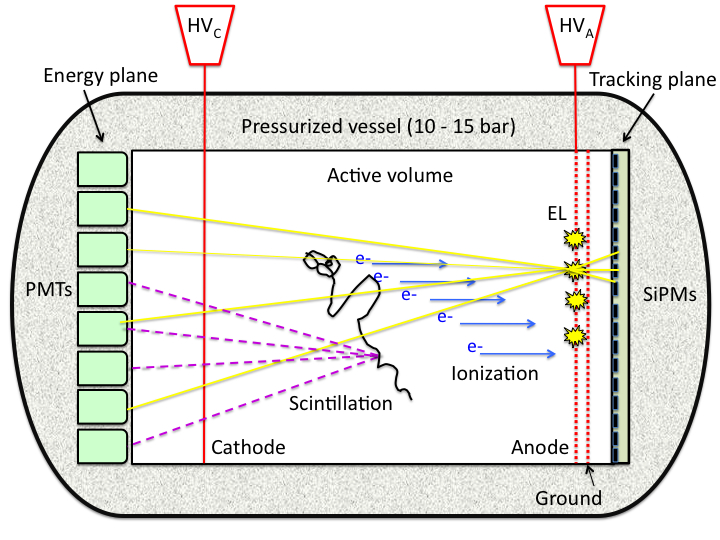
\includegraphics[width=0.49\textwidth]{img/SOFT.jpg}
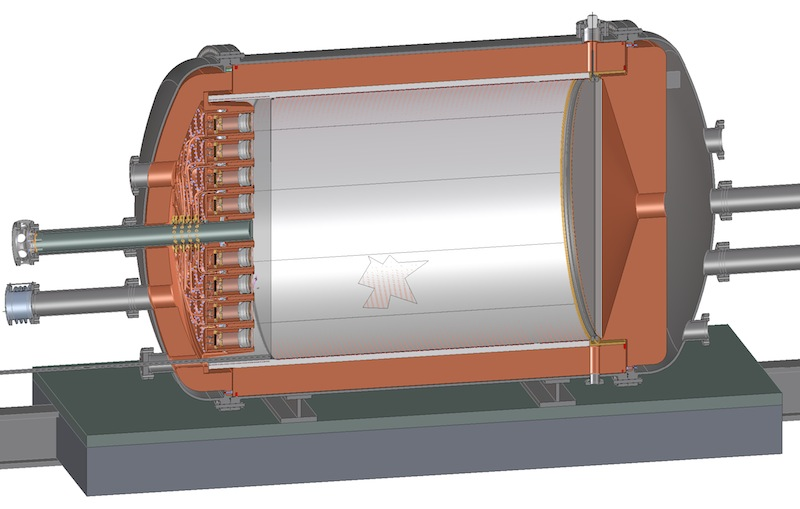
\includegraphics[width=0.49\textwidth]{img/NEXT100_full.jpg}
\caption{\small Left: The detection process in NEXT. Right: cross-section drawing of the NEXT-100 detector. The pressure vessel, 2.3 m long and 1.5 m diameter, can hold up to 150 kg of xenon at 15 bar.} \label{fig.SOFT}
\end{figure}
%%%%%%%%%%


The design of the NEXT-100 detector, shown in the right panel of Figure~\ref{fig.SOFT}, has been published in a \emph{Technical Design Report}.\footcite{Alvarez:2012haa} The construction of the detector ancillary systems (shielding, gas system, etcetera) is underway at the Laboratorio Subterr\'aneo de Canfranc (LSC), in Spain. 

NEXT-100 has the structure of a Matryoshka (a Russian nesting doll). The outermost layer is a shield made of lead, which attenuates the background from the LSC rock by 6 orders of magnitude (e.g, the \TL\ photons are attenuated from $\sim 10^{12}$~per year to $\sim 10^{6}$~per year). The pressure vessel, built out of steel, can hold 150 kg of xenon at 15 bar. Finally, an inner copper shield, 12 cm thick, constitutes the innermost and more radio-clean layer of the Matryoshka. All NEXT components have been selected and screened for low background. Of particular importance are the PMTs, whose activity is only 0.4 mBq of \BI\ and 0.3 mBq of \TL\ per unit. Our TDR shows a full quantification of the different contributions to the NEXT radioactive budget. A recent paper\footcite{Alvarez:2012as} quantifies the results of our screening campaign. Currently, most of the major components entering the NEXT detector have been measured, and those numbers are incorporated in our background model. 


\subsubsection*{Discovery potential}

%%%%%
\begin{figure}
\centering
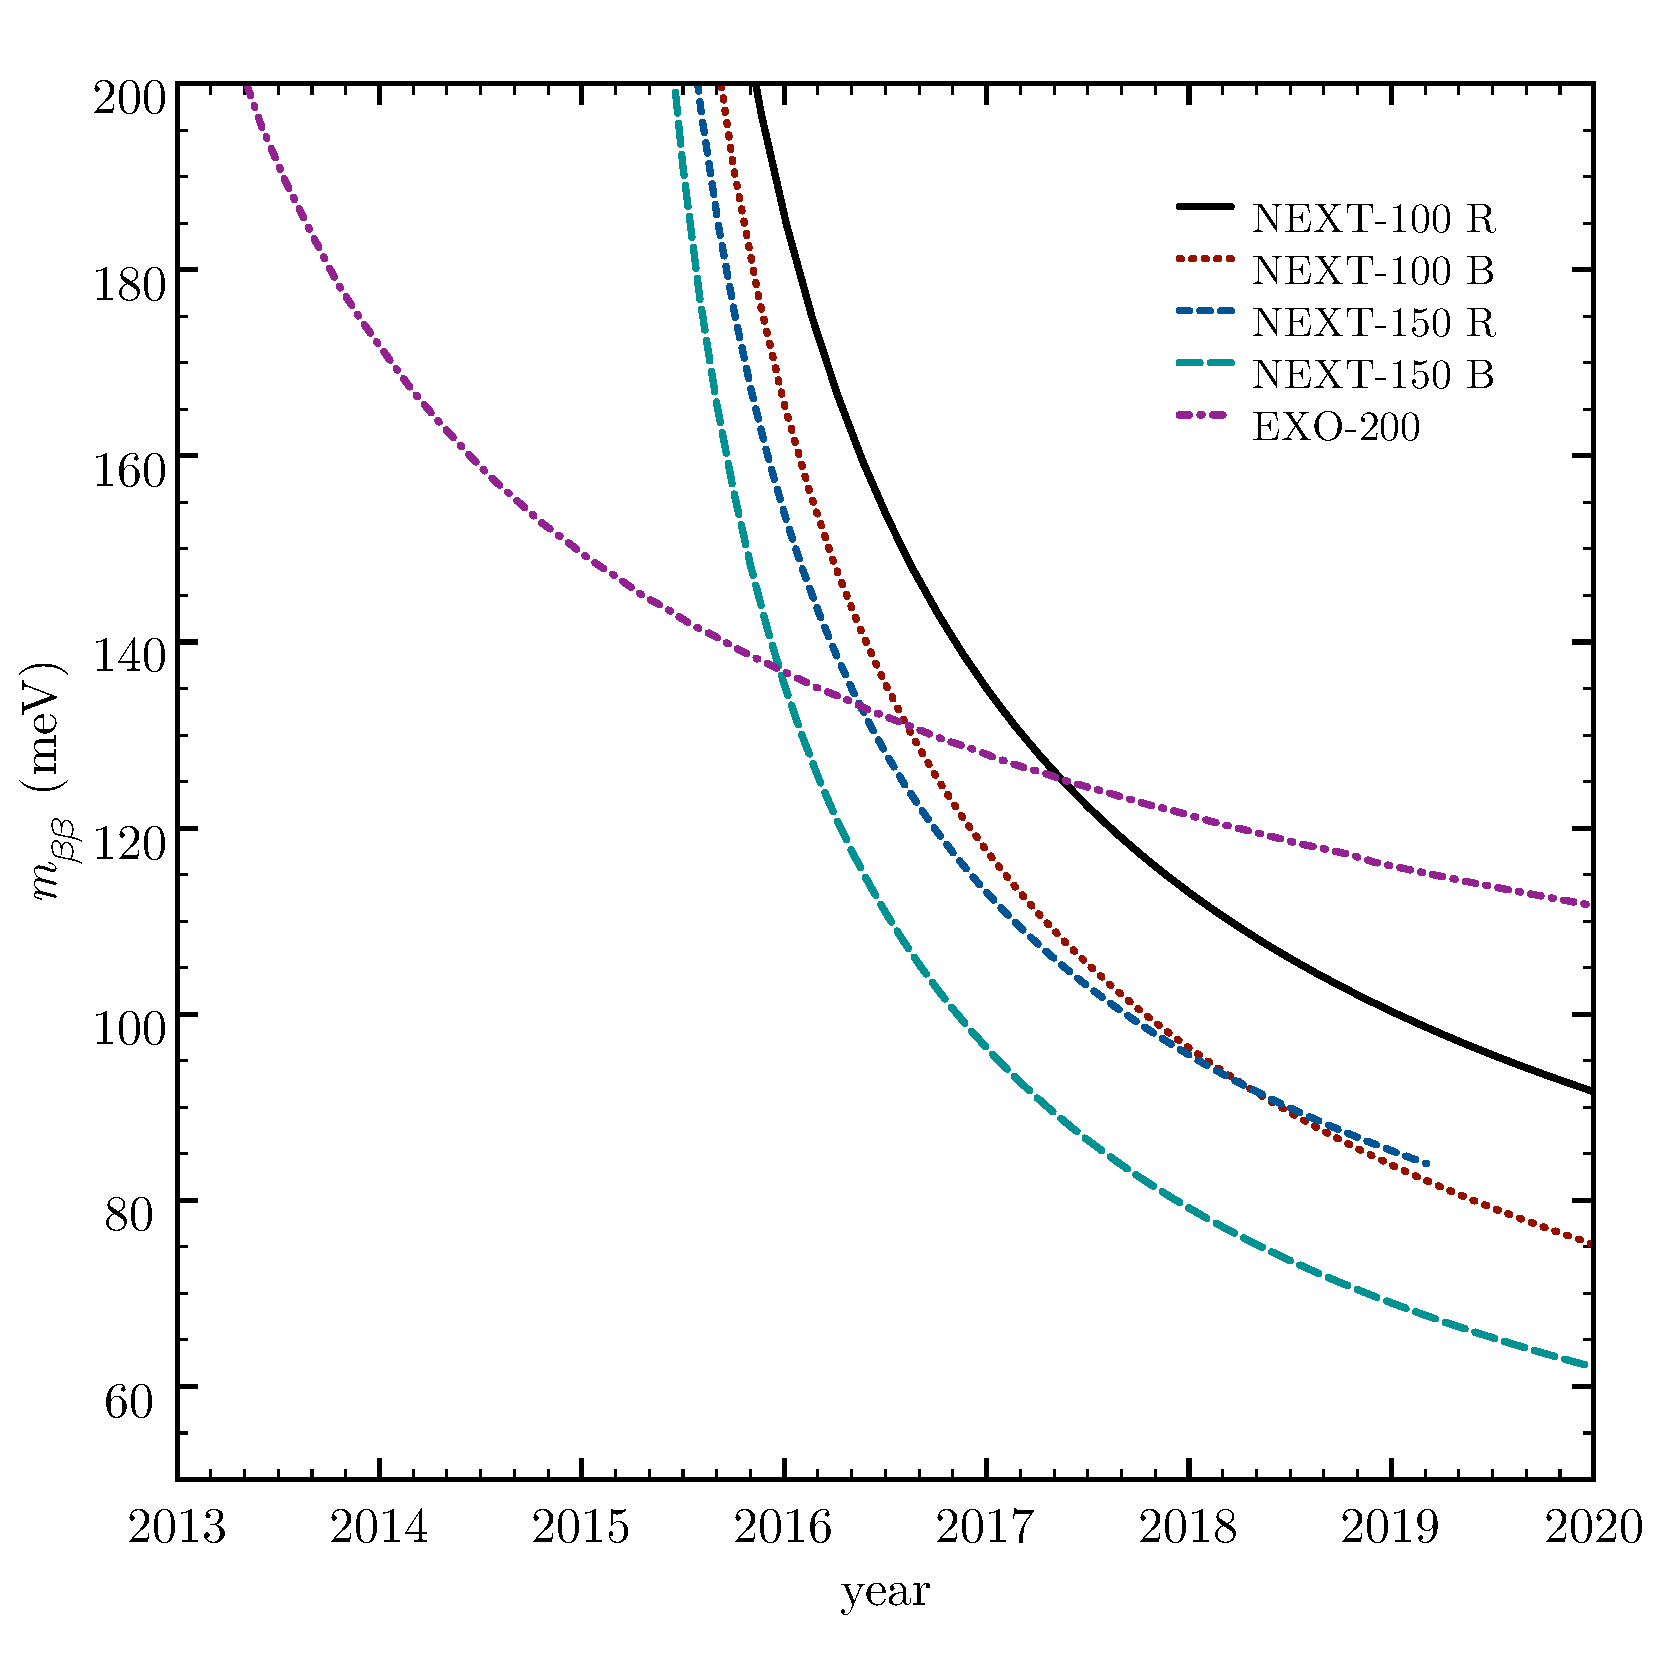
\includegraphics[width=0.5\textwidth]{img/EXOvsNEXT2.pdf}
\caption{Sensitivity of NEXT-100 assuming reference (R) and best (B) scenarios described in the text, as well as 100 and 150 kg of isotope mass.  The sensitivity of EXO-200 is drawn also for reference. It is assumed that the NEXT-100 \emph{physics run} starts in mid 2015.} \label{fig.exoNext}
\end{figure}
%%%%%

As shown in our TDR, the combination of excellent energy resolution and topological signature, results in a very good background rejection factor, estimated to be $\sim 2 \times 10^{-7}$~for the dominant background channels (the Bi-214 and Tl-208 
gammas of high energy entering the detector). NEXT-100 is a very radio-clean detector, protected by a thick shield of ultra radio pure copper, using ultra-radio pure PMTs and MPPCs. This, combined with the good background rejection factor, results in a very low background rate.

As a consequence, the discovery potential of NEXT is large. As explained below, we assume that the physics run starts in mid  2015, after detector commissioning in 2014. In our TDR we assumed a resolution of 1\% FWHM and quoted a background rate of $8 \times 10^{-4}$~\ckky, obtained from a detailed Monte Carlo calculation using our full background model. Since publication of the TDR our prototypes have measured better resolution than that assumed. DEMO reaches 0.8\% FWHM in a large fiducial volume, while DBDM reaches 0.5\% in a more restricted fiducial region. Moreover, the background model is fully backed by an extensive screening campaign that has fully quantified the radioactivity of all the components entering the detector\footcite{Alvarez:2012as}.

Indeed, as explained in the next sections, we believe that both figures can be improved. We aim, as a part of the research program described in this proposal, to achieve a resolution of 0.5\% FWHM at \Qbb, in the full fiducial region and a background rate of 
$2 \times 10^{-4}$~\ckky. The possibility exists to operate the detector with 100 kg of Xe-136 (already available) at 10 bar, or with 150 kg of Xe-136 at 15 bar.

Figure \ref{fig.exoNext} shows the sensitivity of NEXT-100 from the start of physics data taking under four scenarios: (a) reference,  with the conservative parameters assumed in the TDR and 100 kg of isotope in the chamber; (b) reference, with 150 kg of xenon; (c)  best, with the improved parameters described above and 100 kg of xenon; (d) best with  150 kg of isotope. For reference, we also consider the sensitivity of EXO-200, assuming the parameters described in the recent publication \footcite{Auger:2012ar}. 

Notice that the discovery potential of NEXT-100, in particular with 150 kg and/or the improved parameters is very high. Currently, EXO-200 and KamLAND-Zen are dominated by backgrounds and therefore, further data taking without detector improvement will yield a slow improvement in their results. Thus, in spite of a relatively late start, NEXT could quickly become competitive.  On the other hand, if GERDA, EXO-200, KamLAND-Zen
or another experiment (such as CUORE) were to claim a discovery in the next few years, NEXT would be in the perfect position to provide an independent confirmation.  

\subsubsection*{Towards a ton-scale HPGXe TPC}

%%%%%%
%\begin{figure}
%\centering
%\includegraphics[width=0.65\textwidth]{imgs2/SensitivityFuture.pdf}
%\caption{The sensitivity of NEXT versus that of EXO in the 1-ton regime.} \label{fig.NextFuture}
%\end{figure}
%%%%%%

If no discovery is made by the current generation of experiments, the full exploration of the inverse hierarchy of neutrino masses requires detectors of larger mass (at least 1 ton), with good energy resolution and extremely low specific background. With a resolution of 0.5\% FWHM and a background rate of $2 \times 10^{-4}$\ckky, as we intend to demonstrate in this research, an HPXe detector with a mass in the ton scale could fully explore the inverse hierarchy. %The discovery potential is, therefore, enormous. 

In that sense, NEXT is the perfect springboard for a detector in the ton scale. The resolution and background rate described in our TDR would allow a detector of 100-150 kg to reach sensitivities in the range of 50-100 meV, but the improved parameters that we expect to reach after our R\&D, would demonstrate that the HPXe gas technology can fully explore the inverse hierarchy. 

Taking into account that EXO-200 operates in USA and Kamland-Zen operates in Japan, the NEXT program offers a unique opportunity for Europe to lead with the HPXe technology. This would make Europe a major player in the area of xenon detectors applied to \bbonu. This is particularly relevant, since xenon will very likely be the easiest isotope to reach the ton scale.
 
